\documentclass[hyperref={pdfpagelabels=false},12pt]{beamer}
\usepackage[utf8]{inputenc}
%\usepackage{multirow}
%\usepackage{wasysym}
%\usepackage{upquote}
\usepackage{listings}
\usepackage{gensymb}
\usepackage{array}
\usepackage{times}
\usepackage{xcolor}
\usepackage{default}
\usepackage{ulem}

%\usetheme{Pittsburgh}

\xdefinecolor{darkgreen}{rgb}{0.11,0.64,0.22}
\title[Pitt Access]{{\large Pitt-ACCESS\\ A Comprehensive and Critical Evaluation System for Software}}
\author[Pitt-Access]{{\scriptsize \textbf{Ketan and Barry}}}
\date{}

\beamertemplatenavigationsymbolsempty


\begin{document}
\begin{frame}[plain]
\titlepage
\end{frame}

%Introduction
\begin{frame}
\frametitle{Motivation: Why do we want to do this?}
\begin{itemize}
\itemsep1em
\item 
Frustration with science software: architectures, installation, runtime, maintenance, dependencies, platforms, libraries, tools, compilers
\item 
Lack of an independent, neutral and critical evaluation platform: quantitative and qualitative
\item 
Benefit from a strong science software: applications, tools, techniques, technology
\end{itemize}
\end{frame}

\begin{frame}
\frametitle{Details: What Pitt-ACCESS is all about?}
\begin{itemize}
\itemsep1em
\item 
A platform to \textbf{critically} evaluate science software: applications, tools, libraries, compiler suites, standards and implementations.
\item 
Answers to questions such as:
\begin{itemize}
\item 
I need an MD software for the Nvidia/CUDA platform, which one is the best?
\item 
Does the new combustion engine simulation software run over IBM BlueGene architectures?
\item 
Is it worth buying the latest compiler suite from PGI?
\item 
How well does \textit{VASP} scale for 750 ion problem space?
\end{itemize}
\end{itemize}

\end{frame}

\begin{frame}
\frametitle{Architecture: What are the components of this framework?}
\begin{itemize}
\item 
Layered architecture: User Interface (web portal), Test Framework, Evaluation Framework, Database, Storage
%\item
%User accounts management system: community contributes, reviews and rates
%\item
%Catalog: tag and locate
%\item
%Structured database for contents
\end{itemize}
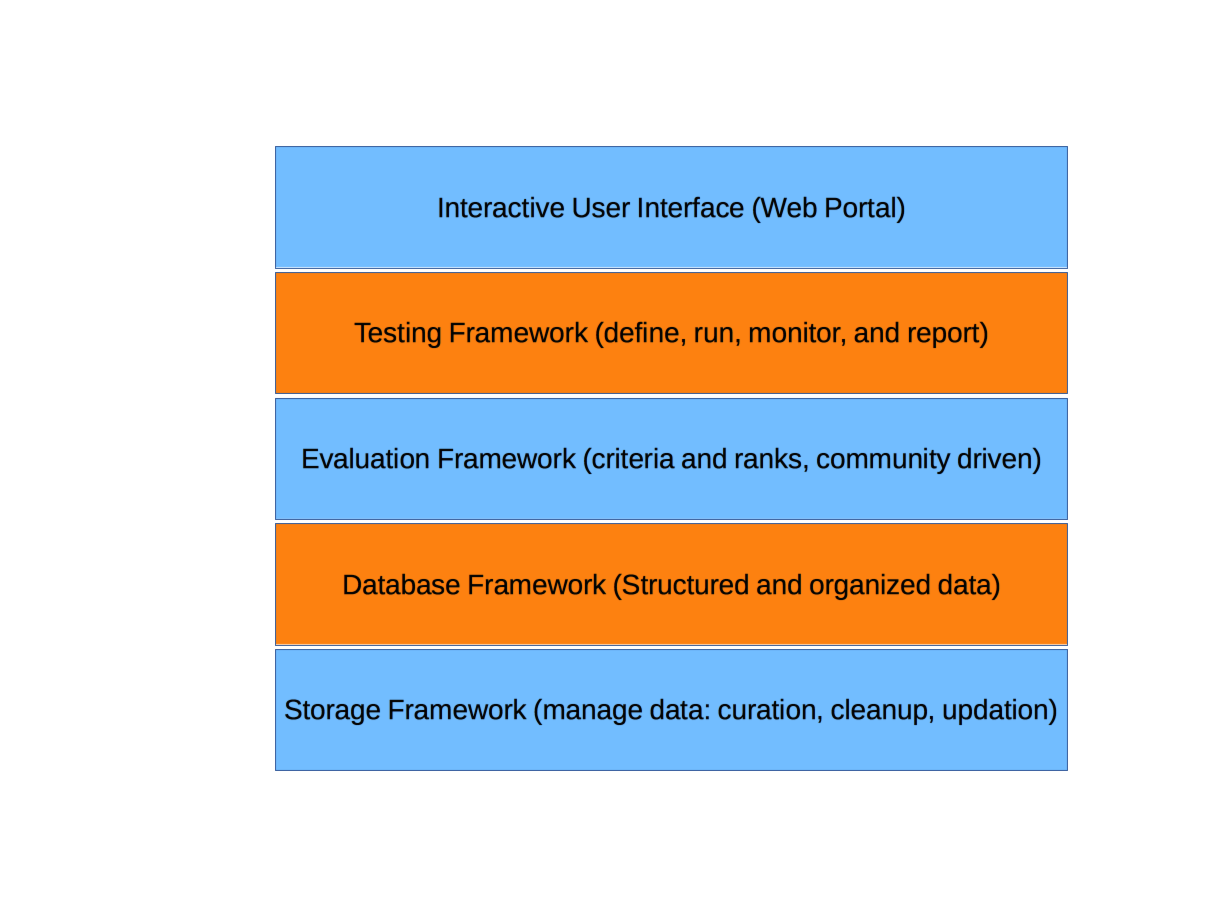
\includegraphics[width=9.6cm]{Architecture}
\end{frame}

\begin{frame}
\frametitle{Execution: Automated workflow}
\begin{center}
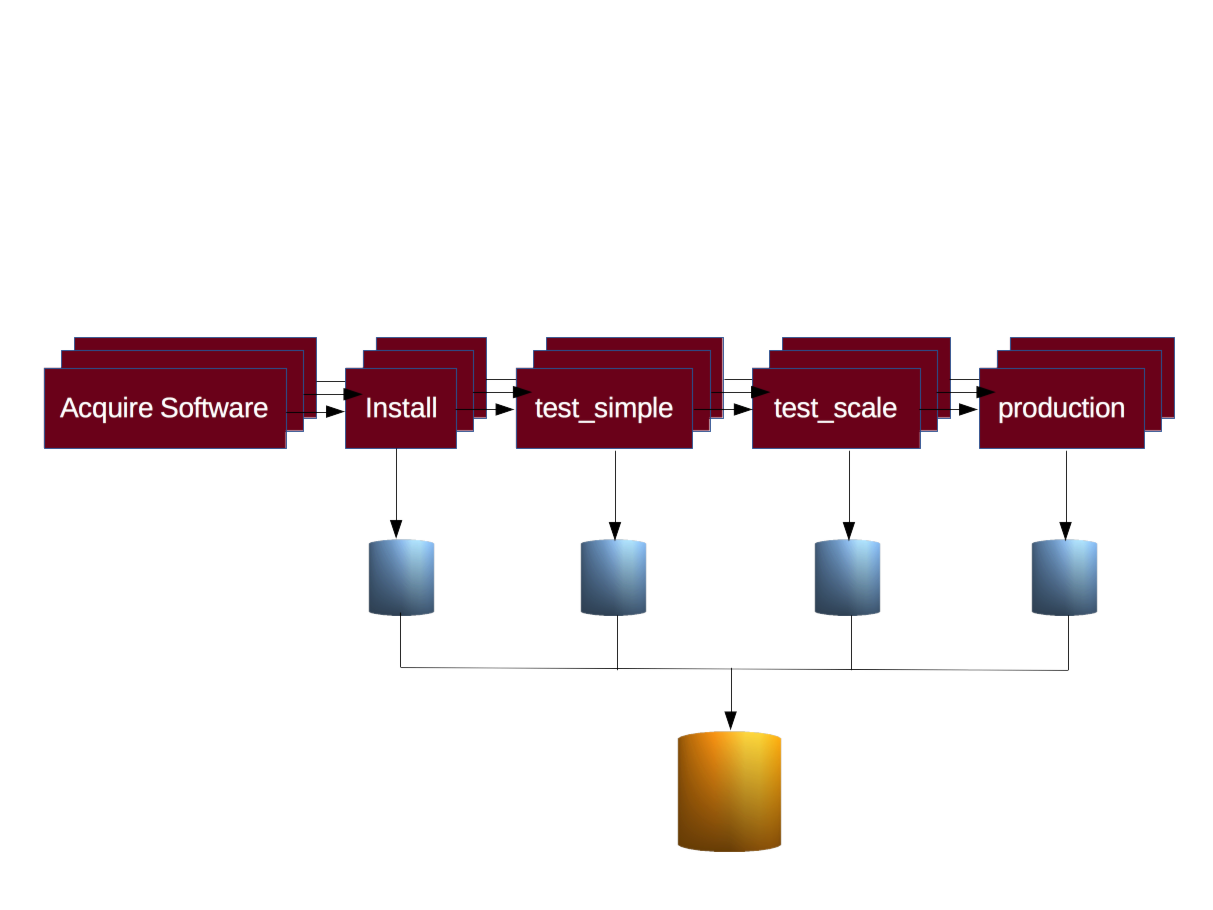
\includegraphics[width=11cm]{workflow}
\end{center}
\end{frame}

\begin{frame}
\frametitle{Challenges: potential roadblocks}
\begin{itemize}
\itemsep1em
\item
 Sustainability: How do we sustain the effort?
\item 
Strategic: potentially making important people upset
\item
Technological: design, web development
\item
Legal: licensing issues, what to publish and what to withold (start with ``local" software)
\item
Unforeseen: this is a unique and first of its kind effort! (I know everyone says so!)
\end{itemize}
\end{frame}

\begin{frame}
\frametitle{Benefits: What are the benefits?}
\begin{itemize}
\itemsep1em
\item Strengthen SaM's (and Pitt's) software platforms
\item
Saves time and money for SaM as well as their users
\item
Strong community outreach elements
\item
Deeper understanding of science software leads to better collaboration
\item 
Better information of what the community is up to
\item
Keep in touch with leaders/PIs and vice versa
\item
Discover new bugs and improve quality
\end{itemize}
\end{frame}

\begin{frame}
\frametitle{Example results(1): comparative view of apps}
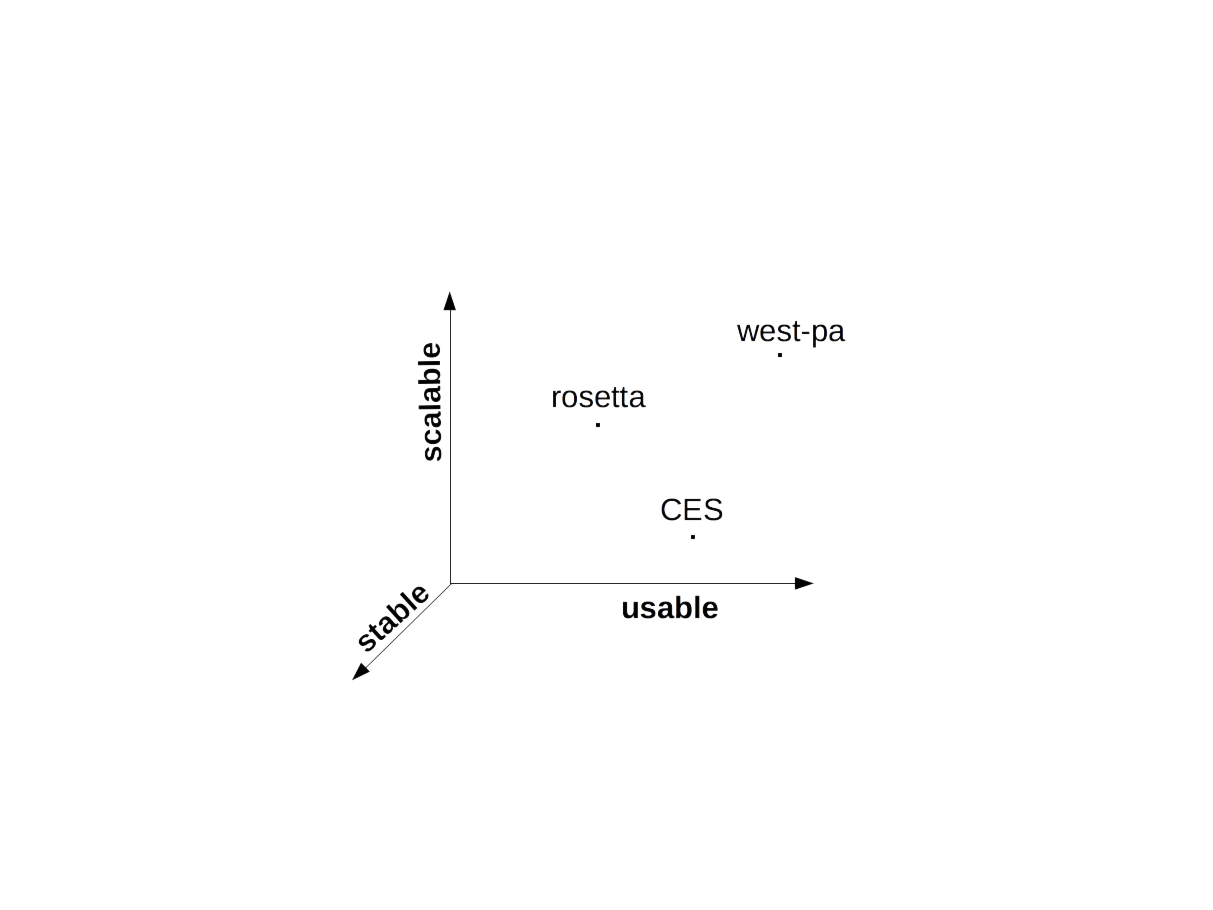
\includegraphics[width=9cm]{example1}
\end{frame}

\begin{frame}
\frametitle{(2): app vs compiler over a \textit{Dell cluster}}
\begin{table}
\begin{center}
% use packages: array
\begin{tabular}{|c|c|c|c|c|c|}
\hline
\textit{comp/app} & \textbf{ipopt} & \textbf{VASP} & \textbf{rosetta} & \textbf{dock} & \textbf{icenine} \\
\hline
\textbf{Intel Suite} & \checkmark & \checkmark & x & \checkmark & \checkmark \\
\hline
\textbf{GCC} & x & \checkmark & x & x & \checkmark \\
\hline
\textbf{PGI} & x & \checkmark & \checkmark & \checkmark & x \\
\hline
\textbf{clang} & \checkmark & x & x & \checkmark & x \\
\hline
\end{tabular}
\end{center}
\end{table}
\end{frame}

\begin{frame}
\frametitle{Is it well-aligned to SaM's mission? \\ (Why yes ... yes it is!)}
\begin{itemize}
\itemsep1em
\item 
Promote multi-disciplinary research
\item
Enrich knowledge base
\item
New funding opportunities
\item
Long term: leave a mark!
\end{itemize}
\end{frame}

\begin{frame}
\frametitle{Plan: Timeline of activities }
\begin{itemize}
\itemsep1em
\item 
Quarter1-2: design, test, feedback
\item
Quarter 3: Narrow down scope, short term goals, select target software, first webpage goes live
\item
Quarter 4: Add more software, diversify science domain
\item
Select 2-3 software apps
\item
Perform the acquire, install, test, run, scale cycle
\item
Identify and register patterns, eg. effort to install
\item
Tools to build the platform: django/flask?, sqlite3?, json?, ...
\end{itemize}
\end{frame}

\begin{frame}
\frametitle{Summary}
\begin{itemize}
\itemsep1em
\item IMDb of science software!
\item
Valuable at all scales, many fringe benefits
\item
Broader, deeper community engagement and outreach
\item
Contribution to multi-disciplinary software infrastructure
\item
Future: establish a ``center"
\end{itemize}
\end{frame}

\begin{frame}
\frametitle{Questions?, Comments?}
\begin{itemize}
\item We are looking for critical comments and feedback!
\end{itemize}
\end{frame}

\end{document}

